\section{Results}
\label{sec:results}
Physical and estimator checks are followed by a seeded controlled learning study. \pending{Full matched-cost comparisons, flagship design benefits and generalization remain to be established; no abandoned historical result is imported.}
\subsection{Seeded Controlled Learning}
Seven fixed-information arms each completed 64 updates for ten paired training seeds from the same legal SFT checkpoint. Evaluation used the two fixed validation tasks at the five declared checkpoints; every attempted outcome was retained. Initial sampled rewards agree across arms within each seed. Figure~\ref{fig:controlled-fixed} reports the terminal paired effects alongside the actual charged cost, without selecting a checkpoint by its reward.

\begin{figure*}[t]
\centering
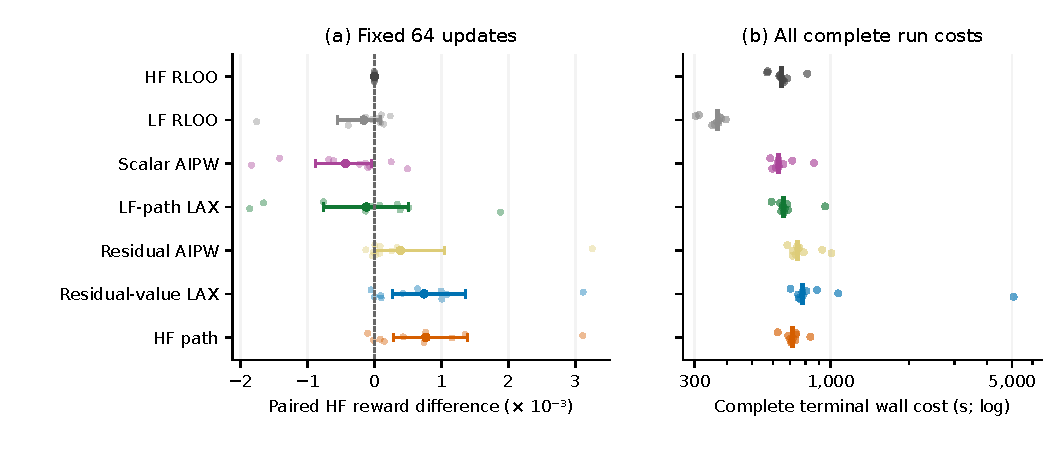
\includegraphics[width=0.98\textwidth]{figures/controlled_fixed_updates.pdf}
\caption{Controlled study at 64 updates, ten paired seeds and two fixed validation tasks. Left: reward difference from HF RLOO; small dots are seed differences, large dots are their means, and bars are descriptive pointwise 95\% paired-seed bootstrap intervals. Right: complete charged wall time for the corresponding runs, including setup, retained failures and target verification; bars indicate medians. This is an update-matched comparison, not a common-wall-budget frontier.}
\label{fig:controlled-fixed}
\end{figure*}

The HF-path and residual-value LAX arms improve the mean terminal target reward relative to HF RLOO in this controlled study. Their paired descriptive intervals lie above zero in Fig.~\ref{fig:controlled-fixed}. The improvement occurs in the thermal component while the analytic control contribution remains close to the reference. These intervals describe variation over the ten training seeds on the fixed tasks; they are not simultaneous tests or evidence of population-level task generalization. The residual-value arm uses a fixed positive acquisition probability and coefficient, and does not test the full adaptive ISPO controller.

The complete information controller has also completed all registered training seeds. Its sampled initial policies agree with the common HF-RLOO start in every seed. At the fixed terminal update, its mean target reward moves positively relative to HF RLOO, primarily through the thermal component; the descriptive paired interval still includes zero. All validation outcomes are retained and independently reconstructed from the original target states. This supports the completed controlled learning experiment while leaving the matched-cost comparison and the full moving-policy information study to be established.

\subsection{Information Value and Cost--Quality Frontier}
For the seven-arm study, the registered strict common-wall-time interval is empty: one recorded model-loading phase exceeds the shortest completed trial. Its delay and all other costs remain in the cohort. Consequently, Fig.~\ref{fig:controlled-fixed} supports the fixed-update comparison only; no cost-frontier advantage is inferred from it. Controlled admission and the complete method comparisons remain necessary for the main efficiency study.
\pending{Matched-budget comparisons; signal costs; randomized acquisition; complete component ablations; broader layout, data-center and aerodynamic validation.}

\subsection{Information Mechanisms}
The controlled finite-volume evaluator supplies a verified physical reference for separating information effects from implementation errors. Directional derivatives, conservation and boundary-response checks establish its declared residual and sensitivity routes. Complete policy-parameter reconstruction supports the corrected value/path assembly. Detailed native-array and interface evidence is retained in the supplementary material.

\subsubsection{Objective-aware residual feedback}
A preregistered set of 60 designs was evaluated at both cavity fidelities, with all attempted outcomes and costs retained. On its 12 predeclared diagnostic anchors, the adjoint-weighted correction was constructed using only the interpolated coarse state and the exact target operator, without a target forward solve or use of target fields. The target scalar was read only after prediction persistence for independent post-validation. Table~\ref{tab:goal-correction} separates the correction's numerical effect from its acquisition cost.
\begin{table}[t]
\centering
\caption{Bounded goal-correction mechanism on 12 predeclared cavity designs. Errors concern the common thermal objective, not field error.}
\label{tab:goal-correction}
\begin{tabular}{lr}
\toprule
Quantity & Measured value \\
\midrule
Mean absolute coarse-goal error & $2.5171\times10^{-3}$ \\
Mean error after target-grid mapping & $2.1311\times10^{-3}$ \\
Mean error after adjoint correction & $2.0240\times10^{-4}$ \\
Largest transpose relative residual & $2.25\times10^{-13}$ \\
Largest directional FD relative error & $2.05\times10^{-8}$ \\
Correction work, 12 designs (s) & $5.76$ \\
Additional one-time setup (s) & $4.63$ \\
\bottomrule
\end{tabular}
\end{table}
The raw or fixed-block-scaled residual norms did not positively rank the original thermal-goal error on these anchors. The absolute predicted total goal discrepancy from the adjoint construction had positive rank association with that same error. This distinction motivates the objective-aware interface: the useful signal estimates the quantity being optimized rather than assuming that an aggregate equation norm is sufficient. No total-budget learning gain is inferred from the correction table; mapping, Jacobian, transpose-solve and setup charges remain in the acquisition ledger.


\subsubsection{Information-guided parameter updates}
A fixed-policy study stores complete trainable-parameter gradients for fresh physical design groups, using separate past groups to calibrate coefficients. Predictably calibrated path controls reduce within-context target-gradient variation. Fixed coefficients can instead amplify it, explaining why information content alone does not determine update quality. Exact acquisition-mask enumeration verifies the conditional moment calculation. The collection, calibration and recording costs remain charged; these mechanism results motivate the complete moving-policy cost comparison rather than replacing it.

\subsection{Policy and Training Economy}
The structured-policy study completes both registered update recipes for ten seeds from a common supervised start. Both improve over that start in every seed. Continuous LAX reaches similar fixed-terminal target quality to HF RLOO while using fewer target calls and lower mean complete training cost (Fig.~\ref{fig:e5-terminal}). Native objective decomposition explains the close quality result: its thermal improvement is offset by increased actuator cost. The checked gradients and objective decomposition identify the thermal/control tradeoff in this experiment. The complete controller and registered ablations will test how additional information changes that tradeoff.

\begin{figure*}[t]
\centering
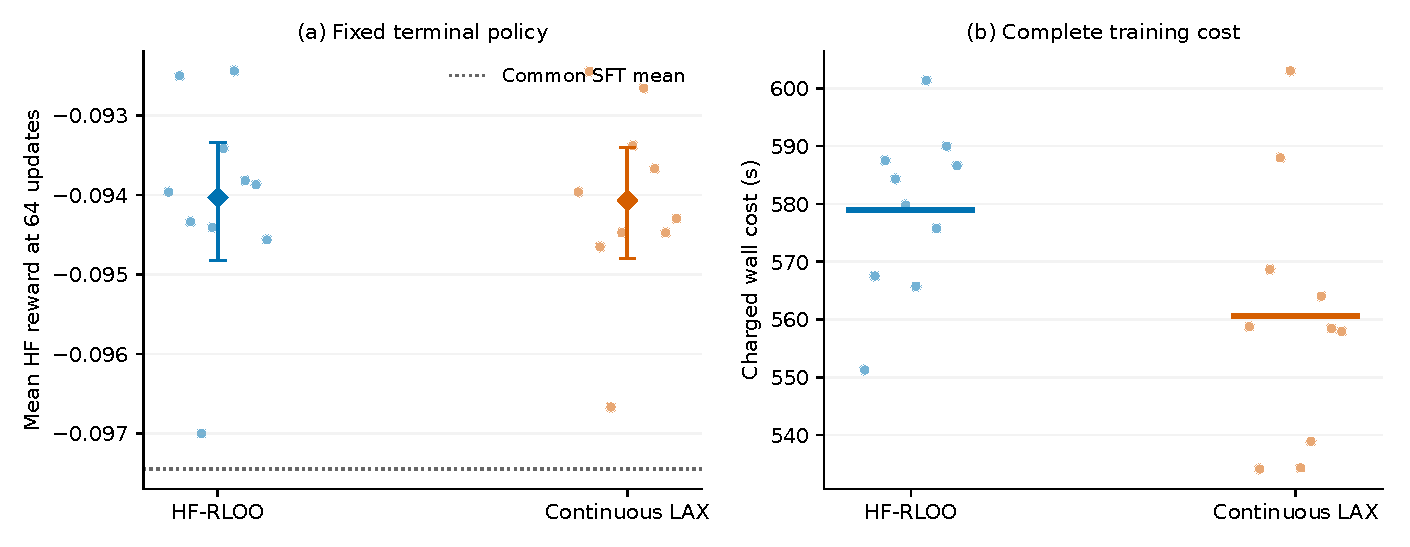
\includegraphics[width=\textwidth]{figures/e5_structured_terminal.pdf}
\caption{Complete structured-policy study at the registered 64-update checkpoint. Dots retain every training seed; diamonds and error bars show means and descriptive 95\% seed-block intervals. The dotted line is the common SFT mean. Right-panel costs include model initialization, actual physical calls, updates, recording and terminal process closure.}
\label{fig:e5-terminal}
\end{figure*}

The predeclared E5 comparison combines the same two recipes across the language and structured policies, retaining all forty trials. Its common charged-cost interval supports an actual matched-cost comparison (Fig.~\ref{fig:e5-frontier}); the original seven-arm study's empty interval is unchanged. The language and structured curves have overlapping descriptive intervals toward the end of this interval. This compares the registered architectures and recipes, including their distinct initialization weights and learning rates; it does not establish a universal preference for a model class. All terminal structured policies have now completed actual deployment, project export and target verification on both public validation contexts. Every first and repeated request is retained, and independent reconstruction from the native high-fidelity state and archived cell volumes confirms the objective components. Cold model and evaluator preparation, complete command costs and warm request costs are recorded separately. The workload calculation includes inference, export and paid verification alongside training. The registered per-task study has also completed all four native optimizers across six tasks and ten seeds. Independent reconstruction verifies every physical call, target-eligible incumbent and complete trial cost. Together with the measured policy deployment, this supplies the reference experiments for the amortization study. The trained policies improve over the registered midpoint rule on both validation contexts for every model seed. Actual language-policy deployment and the quality-matched comparison with the complete optimizers remain the next experiments.

\begin{figure*}[t]
\centering
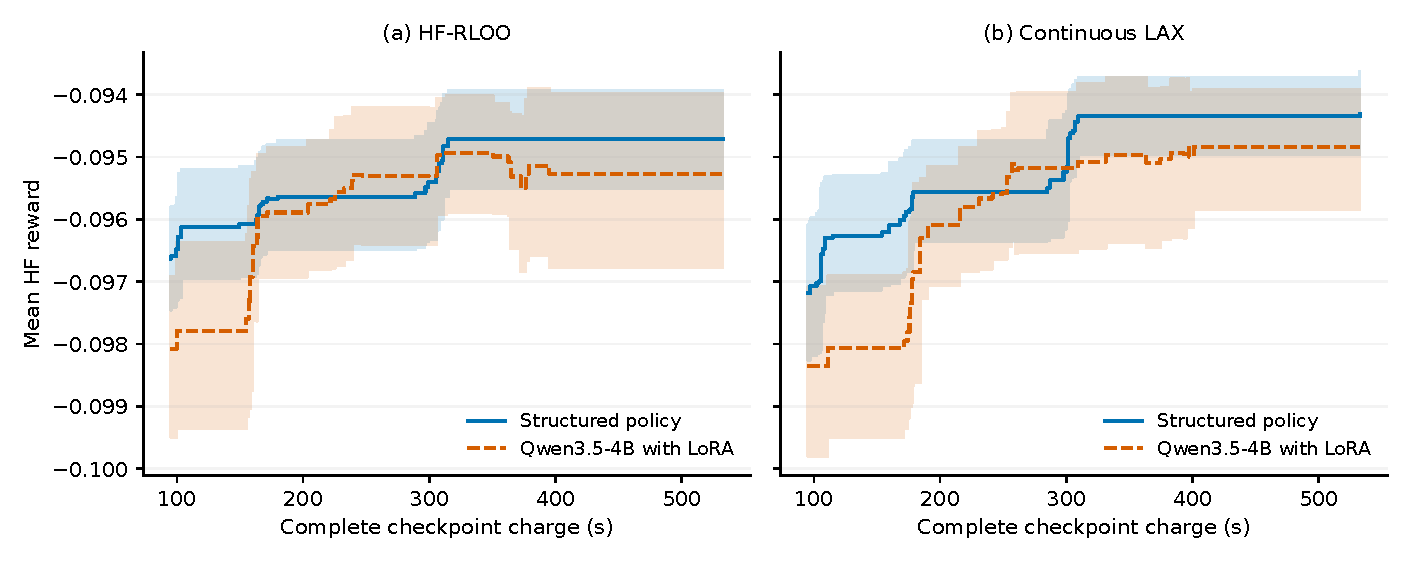
\includegraphics[width=\textwidth]{figures/e5_architecture_frontier.pdf}
\caption{Predeclared E5 comparison on two fixed validation contexts. Each panel uses ten seeds per architecture and the corresponding registered update recipe. The latest affordable checkpoint is evaluated at each charged budget; there is no reward-based checkpoint selection, interpolation or extrapolation. Bands are descriptive pointwise 95\% seed-block mean intervals. Architectures use common requirements and heuristic labels with distinct SFT weights and registered learning rates.}
\label{fig:e5-frontier}
\end{figure*}

The source-explicit original-task MFPG reproduction completes the full seed cohort and supports its improvement over HF-only. Supplementary Material retains its complete curves, native coupling, evaluation isolation and cost evidence. This provides an implementation anchor for the strong-baseline study. The subsequent MFPG-PPO comparison uses the shared physical design objective and the baseline's native surrogate, coupling and allocation mechanism.

\subsection{Flagship and Aerodynamic Evidence}
The Shinaide references establish joint low-fidelity evaluation for the compiled architecture families. All six references are feasible in normal operation and every registered single-unit outage under the synthetic task constraints. Every original context is retained, including the recorded startup failure and its source-only logging repair. Each candidate binds the original server inventory, fan-assisted heat budget and liquid topology to both physical branches. Independent native-state reconstruction agrees with per-server enthalpy closure and the complete device/plant electricity account. The perimeter operators consume actual floor apertures, containment and return paths. Interchangeable equipment and shared mixing nodes explain equal responses in symmetric low-fidelity references. Room-CFD checks will establish the location-dependent higher-fidelity response, and learning studies will measure the design benefit.

The supported aerodynamic benchmark verifies the complete sixteen-dimensional raw drag and lift sensitivities at its registered coarse-grid center. Two-step cold-forward differences and independent native adjoint reconstruction pass the original gates after restoring the wall-distance shape dependence. The derivative bridge preserves the original forward solution and distance algorithm. This closes the local aerodynamic gradient interface needed for the wing study; the registered refined-grid and task-domain experiments supply the remaining evidence.

\subsection{Generalization and Design Automation}
\pending{Held-out requirements and geometries; data-center hard-project validation; second-domain evidence; amortization and deployment cost.}
\section{Discussion}
The completed evidence connects the information interfaces to the design-update mechanism. In the controlled task, target sensitivities and the residual-value control improve the thermal part of the fixed-update comparison. Objective-weighted residual feedback also predicts the target-goal discrepancy more usefully than a raw equation norm on the registered anchors. Together, these observations support information stratification: the useful question is how an available physical signal changes the parameter update relative to its acquisition cost.

The structured-policy comparison shows why both objective decomposition and complete execution costs matter. Its two update recipes reach similar terminal quality while allocating physical calls differently. Thermal improvement and actuator cost can partly offset each other, even when the gradients are correctly connected. The cost--quality study therefore retains the fixed checkpoints, original failures and setup costs, and distinguishes a checkpoint's availability from final process closure. The full controller and strong-baseline experiments will test this allocation mechanism as the policy changes.

The engineering interfaces make the scenario suite executable through source-bound projects and physical records. The six mixed-cooling reference families preserve the original server inventory, fan-assisted heat balance and liquid topology, and support the declared normal and outage contexts. The aerodynamic checks establish the total shape-sensitivity route after restoring the wall-distance dependence. These interfaces provide a coherent foundation for the design-automation experiments. The current inputs retain their declared synthetic provenance and steady heat-generation assumptions; subsequent task-domain and higher-fidelity comparisons use the same explicit acceptance contracts.

\pending{Complete the moving-policy matched-cost comparisons, language-policy deployment, broader task-domain evidence and flagship design study before interpreting the full efficiency and generalization claims.}

\section{Conclusion}
ISPO organizes scalar rewards, physical components, residual feedback and sensitivities within a common budgeted post-training formulation. The verified estimators and controlled learning study support the value of connecting physical information to policy-parameter updates, while the objective-aware correction shows how residual information can be tied to the optimized quantity. Source-bound mixed-cooling and aerodynamic interfaces connect this mechanism to the broader design task suite.
\pending{Add the conclusions of the complete controller, matched-budget baselines, deployment and generalization studies after their registered cohorts and final design checks are complete.}
